\chapter{Performance-Messungen der parallelen Implementation}

Das Testsystem ist dasselbe geblieben, wie bei der Performance-Analyse. Diesmal wird allerdings in vielen Benchmarks mehr als ein Knoten beansprucht. Auch die Datensätze und die geladenen Module haben sich nicht geändert. 
\begin{correctmore}
	- Zeiten immer noch IO bereinigt
	- Zeitdiagramme immer noch logarithmisch
\end{correctmore}

\section{Evaluierung der Optimierungen}

\subsection{Parallelisierung}

\begin{correctmore}
	- Simpel: meh
	- auf Bildpaaren:
		- Speedup: 2-5x (geschätzt; ohne mehr nodes)
		- alte Singlecore Variante als Referenz
		- linear mit Anzahl der Nodes bis Anzahl der Bildpaare
		- anschließend Stagnation bis zu 2* Anzahl d. Nodes, weil bis da hin einige CPUs immer noch alleine a einem Bildpaar rechnet und alle anderen auf diesen warten müssen
\end{correctmore}

\begin{center}
	\begin{figure}[htbp]
		\begin{subfigure}[b]{0.45\textwidth}
			\centering
			\includegraphics[width=\textwidth]{pdf/mpi_speedup_exp6}
			\caption{Experiment 6}
			\label{fig:mpi_speedup_exp6}
		\end{subfigure}
		\hfill
		\begin{subfigure}[b]{0.45\textwidth}
			\centering
			\includegraphics[width=\textwidth]{pdf/mpi_speedup_lenses}
			\caption{Lenses}
			\label{fig:mpi_speedup_lenses}
		\end{subfigure}
		\caption{Speedup der \textit{mpi} Implementierung gegenüber des vorgegebenen Python-Codes}
		\label{fig:mpi_speedup}
	\end{figure}
\end{center}

\begin{center}
	\begin{figure}[htbp]
		\begin{subfigure}[b]{0.45\textwidth}
			\centering
			\includegraphics[width=\textwidth]{pdf/mpi_times_exp6}
			\caption{Experiment 6}
			\label{fig:mpi_times_exp6}
		\end{subfigure}
		\hfill
		\begin{subfigure}[b]{0.45\textwidth}
			\centering
			\includegraphics[width=\textwidth]{pdf/mpi_times_lenses}
			\caption{Lenses}
			\label{fig:mpi_times_lenses}
		\end{subfigure}
		\caption{Gesamtlaufzeit der \textit{mpi} Implementierung gegenüber des vorgegebenen Python-Codes}
		\label{fig:mpi_times}
	\end{figure}
\end{center}

\begin{center}
	\begin{figure}[htbp]
		\begin{subfigure}[b]{0.45\textwidth}
			\centering
			\includegraphics[width=\textwidth]{pdf/mpi_advanced_speedup_exp6}
			\caption{Experiment 6}
			\label{fig:mpi_advanced_speedup_exp6}
		\end{subfigure}
	\hfill
		\begin{subfigure}[b]{0.45\textwidth}
			\centering
			\includegraphics[width=\textwidth]{pdf/mpi_advanced_speedup_lenses}
			\caption{Lenses}
			\label{fig:mpi_advanced_speedup_lenses}
		\end{subfigure}
		\caption{Speedup der \textit{mpi-advanced} Implementierung gegenüber der \textit{mpi}-Version}
		\label{fig:mpi_advanced_speedup}
	\end{figure}
\end{center}

\begin{center}
	\begin{figure}[htbp]
		\begin{subfigure}[b]{0.45\textwidth}
			\centering
			\includegraphics[width=\textwidth]{pdf/mpi_advanced_times_exp6}
			\caption{Experiment 6}
			\label{fig:mpi_advanced_times_exp6}
		\end{subfigure}
		\hfill
		\begin{subfigure}[b]{0.45\textwidth}
			\centering
			\includegraphics[width=\textwidth]{pdf/mpi_advanced_times_lenses}
			\caption{Lenses}
			\label{fig:mpi_advanced_times_lenses}
		\end{subfigure}
		\caption{Gesamtlaufzeit der \textit{advanced-mpi} Implementierung gegenüber des vorgegebenen Python-Codes}
		\label{fig:mpi_advanced_times}
	\end{figure}
\end{center}

\subsection{Optimierung von Python Engpässen}

\subsubsection{Nutzen bereits optimierter Funktionen}

\begin{correctmore}
	- Speedup: 2.5x
\end{correctmore}

\begin{center}
	\begin{figure}[htbp]
		\begin{subfigure}[b]{0.54\textwidth}
			\centering
			\includegraphics[width=\textwidth]{pdf/speedups_intrinsics_exp6}
			\caption{Experiment 6}
			\label{fig:speedups_intrinsics_exp6}
		\end{subfigure}
		\hspace{-0.9cm}
		\begin{subfigure}[b]{0.54\textwidth}
			\centering
			\includegraphics[width=\textwidth]{pdf/speedups_intrinsics_lenses}
			\caption{Lenses}
			\label{fig:speedups_intrinsics_lenses}
		\end{subfigure}
		\caption{Speedup der \textit{intrinsics} Implementierungen gegenüber dem vorgegebenen Python-Code}
		\label{fig:speedups_intrinsics}
	\end{figure}
\end{center}

\begin{center}
	\begin{figure}[htbp]
		\begin{subfigure}[b]{0.54\textwidth}
			\centering
			\includegraphics[width=\textwidth]{pdf/speedups_exp6}
			\caption{Experiment 6}
			\label{fig:speedups_exp6}
		\end{subfigure}
		\hspace{-0.9cm}
		\begin{subfigure}[b]{0.54\textwidth}
			\centering
			\includegraphics[width=\textwidth]{pdf/speedups_lenses}
			\caption{Lenses}
			\label{fig:speedups_lenses}
		\end{subfigure}
		\caption{Speedups der einzelnen Implementierungen gegenüber der \textit{intrinsics} Implementierung}
		\label{fig:speedups}
	\end{figure}
\end{center}

\subsubsection{Kompilieren}

\paragraph{Gesamtes Programm}

\begin{correctmore}
	- 1-2\% schneller als intrinsics
\end{correctmore}

\paragraph{numba}

\begin{correctmore}
	- kein speedup
	- cpython compiler besser, da er direkt für python gemacht wurde
	- bereits viel durch intrinsics optimiert
\end{correctmore}

\paragraph{Cython + komplett}

\begin{correctmore}
	- ??? +5\%?
\end{correctmore}

\section{Einfluss der Parameter}

\begin{correctmore}
	- Sweet-Spot: ca. 3*\#Bildpaare
	- skalliert mit mehr Nodes, aber später nicht mehr gut
	- skaliert besser mit mehr Bildpaaren
\end{correctmore}

\section{Skalierung}

\begin{center}
	\begin{figure}[htbp]
		\begin{subfigure}[b]{0.45\textwidth}
			\centering
			\includegraphics[width=\textwidth]{pdf/best_speedup_exp6}
			\caption{Experiment 6}
			\label{fig:best_speedup_exp6}
		\end{subfigure}
		\hfill
		\begin{subfigure}[b]{0.45\textwidth}
			\centering
			\includegraphics[width=\textwidth]{pdf/best_speedup_lenses}
			\caption{Lenses}
			\label{fig:best_speedup_lenses}
		\end{subfigure}
		\caption{Speedup der \textit{compiled} Implementierung gegenüber des vorgegebenen Python-Codes}
		\label{fig:best_speedup}
	\end{figure}
\end{center}

\begin{center}
	\begin{figure}[htbp]
		\begin{subfigure}[b]{0.45\textwidth}
			\centering
			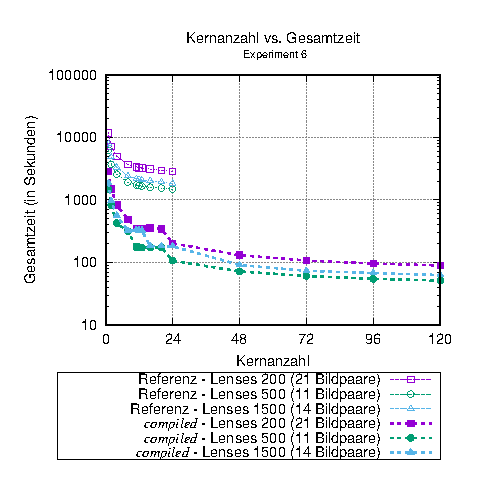
\includegraphics[width=\textwidth]{pdf/best_times_exp6}
			\caption{Experiment 6}
			\label{fig:best_times_exp6}
		\end{subfigure}
		\hfill
		\begin{subfigure}[b]{0.45\textwidth}
			\centering
			\includegraphics[width=\textwidth]{pdf/best_times_lenses}
			\caption{Lenses}
			\label{fig:best_times_lenses}
		\end{subfigure}
		\caption{Gesamtlaufzeit der \textit{compiled} Implementierung gegenüber des vorgegebenen Python-Codes}
		\label{fig:best_times}
	\end{figure}
\end{center}

\subsection{Skalierungsfaktor}

\begin{correctme}
	- schwache skalierung da
	- skaliert aber stark deutlich besser
	- Achtung bei Speedup: 8 Cores als Referenz genommen. wenn bei 8 cores noch kein optimum da ist, kann dass kurz danach gefunden werden, was den Graphen nach obern verschiebt
\end{correctme}

\subsection{Sättigung}

\begin{correctmore}
	- erster Sättigungspunkt bei \#nodes=\#bildpaare, da dann alle CPUs zu 100\% ausgelastet sind --> stagniert bis 2*\#nodes=\#bildpaare
	- neues Bottleneck: Rest des Speckle-trackings (nicht paralleliserter Teil) + Gradientenintegration und nicht parallelisierter Rest der Bildverarbeitungsroutine
	--> nur begrenzte Menge an Daten verfügbar
\end{correctmore}